% REMOVE THIS IN FINAL DRAFT
\renewcommand{\beta}{\gamma}

% Document class
\documentclass{article}

% Packages
\PassOptionsToPackage{usenames,dvipsnames}{color}
\usepackage{amsfonts}
\usepackage{amsmath}
\usepackage{amsthm}
\usepackage{amssymb}
\usepackage{graphicx}
\usepackage{float}
\usepackage{tikz}
\usepackage{multimedia}
\usepackage{dsfont}
\usepackage{braket}
\usepackage{gensymb}
\usepackage{listings}
\usepackage{subcaption}
\usepackage{listings}
\usepackage[autolinebreaks]{mcode}
\usepackage{IEEEtrantools}
\usepackage{courier}
\usepackage{url}

% Colors 
\definecolor{Green}{rgb}{0,.8,.4}
\definecolor{Plum}{rgb}{.5,0,1}

% Theorem environments
\newtheorem{proposition}{Proposition}
\newtheorem{theorem}{Theorem}
\newtheorem{lemma}{Lemma}
\newtheorem{corollary}{Corollary}
\newtheorem{definition}{Definition}
\newtheorem*{remark}{Remark}
\newtheorem*{conjecture}{Conjecture}

% Customized math commands
\newcommand{\hl}{H_\Lambda} 
\newcommand{\hg}{H_\Gamma} 
\newcommand{\xyedge}{x \twoheadrightarrow y}

% Numbering
\numberwithin{equation}{section}
\numberwithin{theorem}{section}
\numberwithin{proposition}{section}
\numberwithin{lemma}{section}
\numberwithin{corollary}{section}
\numberwithin{definition}{section}

\begin{document}

% Title page
\begin{centering}
\thispagestyle{empty}
\large{\textbf{Bound States and Scattering States of a Quantum Particle on Half-Infinite Lattices}} \\
\vspace{5 mm}
\normalsize{by} \\
\vspace{5 mm}
AARON HSU \\
\vspace{5 mm}
Faculty Mentor: Bruno Nachtergaele, Ph.D. \\
\vspace{5 mm}
SENIOR THESIS\\
\vspace{5 mm}
Submitted in partial satisfaction of the requirements for Highest Honors for the degree of \\
\vspace{5 mm}
BACHELOR OF ARTS AND SCIENCES \\
\vspace{5 mm}
in \\
\vspace{5 mm}
MATHEMATICS AND STATISTICS \\
\vspace{5 mm}
in the \\
\vspace{5 mm}
COLLEGE OF LETTERS AND SCIENCE \\
\vspace{5 mm}
of the \\
\vspace{5 mm}
UNIVERSITY OF CALIFORNIA, DAVIS \\
\vspace{5 mm}
%\textcolor{blue}{Final Draft, June 12, 2014}
June 12, 2014

\end{centering}
\newpage

% Table of Contents
\tableofcontents
\newpage

% Abstract
\section*{Abstract}
\addcontentsline{toc}{section}{Abstract}

The motion of a quantum particle, such as an electron, obeys the Schr\"o{}dinger equation, as determined by its Hamiltonian (which corresponds to the total energy of the particle). Such a particle may either remain localized in a small region of space (a bound state) or diffuse through the entire system (a scattering state). We are particularly interested in two-dimensional lattice systems with a boundary, such as a lattice of points in half of the $xy$-plane; physically, this might correspond to a thin layer of atoms on a substrate or to the surface of a crystal. Recent research has revealed that a particle in such a system may either be confined to the boundary in a bound state or diffuse along the boundary. We extend this knowledge by analyzing two configurations that until now have not been studied. Applying techniques of spectral analysis, linear algebra, and functional analysis, we investigate conditions differentiating the two cases and test a conjecture for a general criterion for the existence of a bound state using spectral gaps. We anticipate that our results may find practical applications in the fields of condensed matter physics and materials science and in the design of quantum information devices.

\vspace{\baselineskip}

\noindent{Keywords: \textit{infinite lattices, bound state, scattering state, discrete Laplacian, spectral gap, transfer matrix, boundary conditions, perturbation}}

\newpage

% Section: Introduction
\section{Introduction}

Throughout human history, man has attempted to explain the universe around him, and the progress of much of science, in particular much of physics, can be characterized by attempts to describe the world at an increasingly smaller scale. As a result, to this day, a significant portion of science is dedicated to characterizing matter and describing the manners in which it behaves.

Over the course of time, science has developed successively more refined theories of matter. In 1803, for instance, John Dalton formulated a theory that all matter is composed of atoms. This was followed by discovery of subatomic particles by Pierre and Marie Curie and electrons by J.J. Thomson in 1898. Subsequently, around the turn of the 19th century, Max Planck theorized as to what are now called photons, or quantized packets of light, the particle nature of which was explored by Albert Einstein a few years later.

Following this, Ernest Rutherford demonstrated in 1909 the existence of nuclei in atoms, a model later refined by Neils Bohr in 1913. In 1931, James Chadwick discovered the neutron, and in 1964, Murray Gell Mann and George Zweig proposed the quark model, describing elementary particles even smaller than the subatomic particles of proton and neutron. Recent research has attempted to describe yet smaller components of matter, leading to the development of, e.g., string theory and the theory of loop quantum gravity.

In this paper, however, the matters we are concerned with shall not be quite so small. We consider the kinetic energy of a quantum particle, such as a quark or a lepton, that moves on a system modeled as a finite or infinite integer lattice. In particular, we are interested in two-dimensional lattice systems with a boundary, such as a lattice of points in half of the $xy$-plane. Physically, such a system might correspond to a thin layer of atoms on a substrate or to the surface of a crystal. 

Quantum particles are among the basic building blocks of matter. These particles include the well-known electron, which is an example of a lepton, as well as less well-known leptons, such as muons and neutrinos, in addition to photons, various quarks, and the recently-discovered Higgs boson. The dynamics of such a quantum particle at low energies, i.e., in the non-relativistic regime, are described by the celebrated Schr\"{o}dinger's equation:
	 \[
	 i \hbar \frac{d}{dt} \psi = H \psi.
	 \]
This equation can be solved by diagonalizing the operator $H$ \cite{griffiths}:
	 \[
	 \psi_t = e^{-itH} \psi_0.
	 \]	
This operator is called the Hamiltonian operator and represents interactions between particles in the system; it can be thought of as a sum of matrices, each representing an interaction between two particles or the kinetic energy of a single particle. Quantum particles can reside in one of possibly many energy levels, which are given by the eigenstates of the Hamiltonian.

Quantum particles belonging to a lattice have associated wavevectors residing in a Hilbert space. Specifically, for any given lattice $\Lambda$ with possibly multiple particles belonging to it, the Hilbert space of its wavevectors is
	\[
	\mathcal{H}_\Lambda = \bigotimes_{x \in \Lambda} \mathbb{C}^2.
	\]
In particular, for a one-particle subspace, which we will restrict our attention to in this paper, the Hilbert space is reduced to
	\[
	\mathcal{H}_\Lambda^{(1)} = \ell^2(\Lambda) \cong \mathcal{C}^{|\Lambda|},
	\]
where the $\ell^2$ space is given by 
	\[
	\ell^2(\Lambda) = \{(z_\alpha)_{\alpha \in \Lambda}| z_\alpha \in \mathbb{C}, \sum_{\alpha \in \Lambda} |z_\alpha|^2 < \infty\}
	\]
with the inner product
	\[
	\langle (z_\alpha), (z'_\alpha) \rangle = \sum_{\alpha \in \Lambda} \overline{z}_\alpha  z'_\alpha .
	\]

The Hamiltonian we consider in this paper will initially be the discrete second-order Laplacian operator, which describes the kinetic energy of quantum particles:
\begin{definition}
The second-order Laplacian operator is defined as follows:
	\[
	(H_\Lambda \psi)_x = \sum \limits_{y, |y-x| = 1} (\psi_x - \psi_y)
	\]
where $\Lambda$ is a finite or infinite lattice, $x$ and $y$ denote vertices on $\Lambda$, and $\psi$ denotes the wavevector describing the energy configuration of a particle on the lattice.
\end{definition}

As can be seen from the expression for the operator, we shall only be concerned with nearest-neighbor interactions, i.e., interactions between lattice sites immediately adjoining one another, in addition to each lattice site's inherent energy. This shall remain the case throughout this paper, although we will generalize the relative weights of different interactions in Section 5.

As a remark on notation, in this paper, we will use $\psi_x$ and $\psi(x)$ interchangeably to denote the $x$ component of the wavevector $\psi$, depending on which notation is more clear.

This remainder of this paper is organized as follows. In Section 2, we will consider and solve completely the simplest non-trivial model, the finite one-dimensional ring.  This model will be slightly modified in Section 3, where we will consider the one-dimensional free-end chain and solve the model by employing the technique of transfer matrices.  We will also add a rank-one perturbation to the system and analyze how this changes the Hamiltonian operator's spectral properties. In addition, we consider our first infinite models and analyze their bound states.

We shall then proceed to a two-dimensional lattice in Section 4, then extend it in Section 5 to the entire two-dimensional infinite lattice, which we analyze as a tensor structure of the one-dimensional case. In Section 6, we will state and prove a general theorem providing the existence of a unique zero ground state for general lattices of this type. Relying upon these results, in Section 7, we formulate a conjecture relating bound states of the Hamiltonians considered to their spectral gaps. We test this conjecture in Sections 8 and 9, using the results of Section 5 to inform our analytical and numerical analysis of two different half-infinite lattice models in two dimensions. We close with some discussion of our results and conclusions in the final section.

% Section: A Simple Example: The One-dimensional Ring
\section{A Simple Example: The One-dimensional Ring}

The first lattice $\Lambda$ we consider is a finite, one-dimension joined-end chain of particles.

%Figure: Finite One-dimension Ring

	\begin{figure}[h]
		\centering
		\caption{Finite One-dimension Ring}
		\label{finite1dring}
		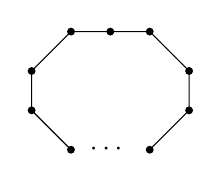
\begin{tikzpicture}
			\draw[thin] (.5,0)--(0,.5)--(0,1)--(.5,1.5)--(1,1.5)--(1.5,1.5)--(2,1)--(2,.5)--(1.5,0);
			\fill (.5 ,0) circle (0.05);
			\fill (0,.5) circle (0.05);
			\fill (0,1) circle (0.05);
			\fill (.5,1.5) circle (0.05);
			\fill (1,1.5) circle (0.05);
			\fill (1.5,1.5) circle (0.05);
			\fill (2,1) circle (0.05);
			\fill (2,.5) circle (0.05);
			\fill (1.5,0) circle (0.05);
			\draw[] (.5,0) -- node[anchor=west] {{ $\cdots$}} (.5,0);
		\end{tikzpicture}
	\end{figure}
	
Our objective is to solve this model by deriving and diagonalizing the Hamiltonian corresponding to $\Lambda$, thereby finding its eigenstates and spectral characteristics. This simple example will also illustrate some basic techniques we will employ in solving subsequent models.

We begin by defining the set of basis vectors that will span the space of wavevectors (i.e., $\ell^2(\Lambda)$) for this matrix:
	\begin{equation}
	\{e_x\}_{x=1}^{n} \text{ where } (e_x)_y = \delta_{xy}.
	\end{equation}

From linear algebra, we know that for any $N$-dimensional inner product space $V$, the elements $(a_{jk})_{1 \leq j,k \leq N}$ of any linear operator $A: V \rightarrow V$, with respect to an orthonormal basis $\{e_j\}$, are given by
	\[
	a_{jk} = \langle e_j, Ae_k \rangle.
	\]
Applying this, we have the following proposition that gives our Hamiltonian:

\begin{proposition}
	The matrix corresponding to the discrete second-order Laplacian operator for the lattice $\Lambda$ (i.e., a one-particle, one-dimensional joined-end chain) can be expressed as follows, in the given basis:
	\label{propham1djoined}
	\begin{equation}
	\label{ham1djoined}
	\\ \hl = \left(
		\begin{array}{cccccc}
			2 & -1 &  &  &  & -1 \\
			-1 & 2 & -1 &  &  &  \\
			 & -1 & 2 &  &  &  \\
			 &  &  & \ddots &  &  \\
			 &  &  &  & 2 & -1 \\
			-1 &  &  &  & -1 & 2 \\
		\end{array}
	\right).
	\end{equation}
\end{proposition}

\begin{proof}
By Definition 1, we have that
\begin{align*}
	\left(H_\Lambda e_j \right) _x &=  \sum \limits_{y, |y-x| = 1} \left( (e_j)_x - (e_j)_y \right) \\
		&= \sum \limits_{y, |y-x| = 1} \left( \delta_{jx} - \delta_{jy} \right) \\
		&= \left\{
			\begin{array}{ll}
				2 & \text{\text{if} } j = x \\
				-1 & \text{\text{if} } j = x \pm 1 \\
				0 & \text{\text{else.}} \\
			\end{array}
			\right.
\end{align*}

Multiplying a basis vector on the left then yields the elements of the matrix:
\begin{equation}
	\left(H_\Lambda \right) _{jk} e_k H_\Lambda e_j = \left\{
		\begin{array}{ll}
			2 & \text{\text{if} } k = j \\
			-1 & \text{\text{if} } k = j \pm 1 \\
			0 & \text{\text{else.}} \\
		\end{array}
		\right.
\end{equation}
\end{proof}

We can diagonalize this matrix with the Discrete Fourier Transform:

\begin{theorem}
	The eigenvalues $\lambda_j$ and eigenvectors $f_j$ of the Hamiltonian operator (\ref{ham1djoined}) are as follows:
	\begin{align}
	\lambda_j &= 2 -2\cos\left(\frac{2\pi i}{M} j\right) \; \; \forall j = 1, \ldots , M \\
	f_j &= (1, \omega^{1 j}, \omega^{2  j}, \ldots, \omega^{(M-1)  j}) \; \; \forall j = 1, \ldots , M.
	\end{align}
\end{theorem}


\begin{proof}	
We observe that this matrix has identical rows that are merely shifted horizontally, i.e., it is a circulant matrix. This allows us to diagonalize it with the Discrete Fourier Transform (DFT) matrix \cite{fenglinetsky}:
	\[
F_M = \left(
	\begin{array}{ccccc}
			1 & 1 & 1 & \cdots & 1 \\
			1 & \omega^{1 \cdot 1} & \omega^{1 \cdot 2} & \cdots & \omega^{1 \cdot (M-1)} \\
			1 & \omega^{2 \cdot 1} & \omega^{2 \cdot 2} & \cdots & \omega^{2 \cdot (M-1)} \\
			\vdots & \vdots & \vdots & \ddots \ & \vdots \\
			1 & \omega^{(M-1) \cdot 1} & \omega^{(M-1) \cdot 2} & \cdots & \omega^{(M-1) \cdot (M-1)} \\
	\end{array}
\right) ,
\]
where $\omega = e^{2 \pi i / M}$ is the primitive $M$-th root of unity.

The diagonalization relation is as follows:
\begin{align*}
	F_M^{-1}\hl F_M &= \Delta
	\\ \Leftrightarrow \hl F_M &= F_M\Delta
	\\ \Leftrightarrow \hl f_j &= \lambda_j f_j \; \; \forall j = 1, \ldots , M,
\end{align*}
writing $F_M = (f_1, f_2, \ldots, f_M)$ and $\Delta = diag(\lambda_m)$.

Therefore, the eigenvectors of $\hl$ are given by the columns of the DFT matrix $F_M$, namely,

\[
f_j = (1, \omega^{1  j}, \omega^{2  j}, \ldots, \omega^{(M-1)  j}) \; \; \forall j = 1, \ldots , M.
\]

The associated eigenvalues are then found as follows:
\begin{align*}
	(\lambda_j f_j)_k &= (\hl f_j)_k \\
	&= 2(f_j)_k - (f_j)_{k-1} - (f_j)_{k+1} \\
	&= 2\omega^{jk} - \omega^{j(k-1)} - \omega^{j(k+1)}.
\end{align*}
We also have that
\begin{align*}
	(\lambda_j f_j)_k &= \lambda_j(f_j)_k \\
	&= \lambda_j\omega^{jk}.
\end{align*}
Setting these expressions equal, we obtain
\begin{align*}
	\lambda_j \omega^{jk} &= 2\omega^{jk} - \omega^{j(k-1)} - \omega^{j(k+1)} \\
	&= 2\omega^{jk} - \omega^{jk} \omega^{-j} - \omega^{jk} \omega^{j}.
\end{align*}

Hence,
\begin{align*}
\lambda_j &= 2 - \omega^{-j} - \omega^{j} \\
	  &= 2 - \cos \left( -\frac{2\pi i}{M}j \right) - i \sin \left( - \frac{2\pi i}{M} j \right) - \cos \left(\frac{2\pi i}{M}j \right) - i \sin \left( \frac{2\pi i}{M} j \right) \\
	  &= 2 -2\cos\left(\frac{2\pi i}{M} j\right)  \; \; \forall j = 1, \ldots , M
\end{align*}
are the respective associated eigenvalues for the eigenvectors $f_j$ previously obtained.
\end{proof}

% Section: The One-dimensional Free-end Chain
\section{The One-dimensional Free-end Chain}

The next class of models we consider are logical variants of the first, where the ends of the chain are no longer joined together (Figure~\ref{1dchain}). We first consider the basic case, i.e., simply removing the interactions between the edge vertices. We then introduce a perturbation to this model at the edge of the lattice.

% Figure: Finite One-dimension Free-end Chain
	\begin{figure}[h]
		\centering
		\caption{A finite one-dimensional free-end lattice	\label{1dchain}}
		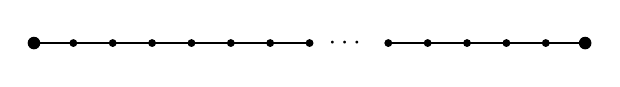
\begin{tikzpicture}
			\draw[thin] (0,0)--(3.5,0);
			\draw[thin] (4.5,0)--(7,0);
			\foreach \x in {0,.5,1,1.5,2,2.5,3,3.5,4.5,5,5.5,6,6.5,7}
				\fill (\x ,0) circle (0.05);
			\draw[] (3.5,0) -- node[anchor=west] {{ $\cdots$}} (3.5,0);
			\fill (0,0) circle (0.08);
			\fill (7,0) circle (0.08);
		\end{tikzpicture}
	\end{figure}

% Subsection: The Basic (No-perturbation) Model
\subsection{The No-perturbation Model}

Following the same method as in Proposition~\ref{propham1djoined} above, it is easy to see that the Hamiltonian for this case is exactly like that in Eq.~(\ref{ham1djoined}), but with no $-1$'s on the lower-left and upper-right corners:
% Array: Hamiltonian for finite one-dimensional free-end chain
	\begin{align*}
	\\ H &= \left(
		\begin{array}{cccccc}
			2 & -1 &  &  &  &  \\
			-1 & 2 & -1 &  &  &  \\
			 & -1 & 2 &  &  &  \\
			 &  &  & \ddots &  &  \\
			 &  &  &  & 2 & -1 \\
			 &  &  &  & -1 & 2 \\
		\end{array}
	\right).
	\end{align*}


	
As a result of the removed elements, the matrix is no longer circulant, and thus, the Discrete Fourier Transform method used in Section 2 can longer be applied. Instead, we apply to the elements of the eigenvectors $v_i$ an \textit{Ansatz} of the form
	\[
	(v_i)_n = \sin(\alpha n + \beta),
	\]
verify that this produces eigenvectors, and solve for acceptable values of $\alpha$ and $\beta$. The eigenvalues follow immediately.

Our results are given in the following theorem:

% Theorem: Eigenstates of the one-dimensional free-end lattice
\begin{theorem}
	The Hamiltonian $\mathcal{H}_\Lambda$ for the one-particle, one-dimensional free-end lattice as described above has eigenvalues $\lambda_i$ and eigenvectors $v_i = (v_i)_{n=1}^N$ as follows:
	\begin{align}
	\lambda_i &= 2 - 2\cos(\beta), \beta = \frac{2 \pi n}{N} \\
	(v_i)_n &= \sin((n-1)\alpha + \beta).
	\end{align}
\end{theorem}

\begin{proof}
	For $n = 2, \ldots, N-1$, i.e., away from the ends of the lattice, we have
	\begin{align*}
	(\lambda_i v_i)_n &= [2 - 2\cos(\beta)] \sin(\alpha (n-1) + \beta) \\
		&= 2\sin(\alpha (n-1) + \beta) \\
		&\hspace{10 mm} - [\sin(\alpha(n-1)+b) \cos(\alpha) - \cos(\alpha(n-1)+b) \sin(\alpha)] \\
		&\hspace{10 mm} - [\sin(\alpha(n-1)+\beta) \cos(\alpha) + \cos(\alpha(n-1)+\beta) \sin(\alpha)] \\
		%&= 2\sin(\alpha (n-1) + \beta) - \sin(\alpha(n-1)+\beta - \alpha) - \sin(\alpha(n-1)+\beta + \alpha) \\
		&= 2\sin(\alpha (n-1) + \beta) - \sin(\alpha ((n-1)-1) + \beta) \\
		&\hspace{10 mm} - \sin(\alpha ((n-1)+1) + \beta) \\
		&= 2\sin(\alpha (n-1) + \beta) - \sin(\alpha (n-2) + \beta) - \sin(\alpha n + \beta) \\
		&= 2(v_i)_n - (v_i)_{n-1} - (v_i)_{n+1} \\		
		&= (\mathcal{H}_\Lambda v_i)_n.
	\end{align*}
	where the third equality uses the sum-difference formula for the sine function.\footnote{The sum-difference formula for sine is:
		\[
		\sin(\alpha \pm \beta) = \sin(\alpha) \cos(\beta) \pm \cos(\alpha) \sin(\beta).
		\]\
	}
		
Note that so far, any values of $\alpha$ and $\beta$ are acceptable. These will be specified by the two boundary conditions.

For $n=1$, the condition we must satisfy is $\hl (v_i)_1 = \lambda_i (v_i)_1$, or
	\begin{equation}
		2\sin(\beta) - \sin(\alpha+\beta) =  [2 - 2\cos(\beta)] \sin(\beta)
	\end{equation}
This equation gives:
\begin{align*}
	\sin(\alpha+\beta) &= 2\cos(\beta)\sin(\beta) \\
	\sin(\alpha+\beta) &= \sin(2\beta) \\
	\sin\left(\alpha + \frac{2\pi n}{N} \right) &= \sin\left(2 \frac{2\pi n}{N} \right) \\
\end{align*}
Therefore, on the boundaries, we have, for $n = 1$:
	\begin{align*}
		(\lambda_i v_i)_1 &= [2 - 2\cos(\beta)] \sin(\beta) \\
			&= 2\sin(\beta) - 2\cos(\beta) \sin(\beta) \\
			&= 2\sin(\beta) - \sin(2\beta) \\
			&= 2\sin(\beta) - \sin(\alpha + \beta) \\
			&= 2(v_i)_1 - (v_i)_2 \\	
			&= (\mathcal{H}_\Lambda v_i)_1.
	\end{align*}
The case for $n = N$ is analogous.
\end{proof}

% Subsection: The Edge Perturbation Model
\subsection{The Edge-perturbation Model}

Next, we add a rank-one perturbation to the model. The notation will be clearer if we generalize the Hamiltonian somewhat by replacing the $2$'s with a variable $b$. To add a perturbation, we further replace the upper-left-most $b$ with a parameter $a$ to determine how this affects the eigenstates of the Hamiltonian. (Physically, this might correspond, for example, to a one-atom impurity on a crystal.) The resulting matrix is as follows:
% Array: Hamiltonian for finite one-dimensional free-end chain, with perturbation
	\begin{align*}
	\\ \hl &= \left(
		\begin{array}{cccccc}
			a & -1 &  &  &  &  \\
			-1 & b & -1 &  &  &  \\
			 & -1 & b &  &  &  \\
			 &  &  & \ddots &  &  \\
			 &  &  &  & b & -1 \\
			 &  &  &  & -1 & b \\
		\end{array}
	\right).
	\end{align*}

We first consider a finite lattice (and hence, a finite operator and matrix), but we are ultimately interested in the behavior of large systems. Accordingly, we will proceed to consider the half-infinite matrix where the bound state(s), if any, of the system will appear, along with the other scattering states.

Because of the asymmetry generated by this perturbation, we employ the transfer-matrix method to find an eigenpair (eigenvalue and eigenvector) for this matrix. We first define the recursive relations that must hold for any eigenvector of $\hl$; these are relatively simple given the tridiagonal nature of the matrix. We express these relations in matrix form and diagonalize this matrix. We then use the diagonalization to find the desired eigenvalue and, from there, proceed to find the eigenvector.



Our results are as follows:

\begin{theorem}
There exists an eigenpair of $\hl$ given by the eigenvalue $\lambda = a - \frac{1}{b-a}$ with the corresponding eigenvector $v = (v_i)_{i=1}^N$, where
\begin{equation}
v_i = \left( - \frac{1}{b-a} \right) ^ {i-1}.
\end{equation}
\end{theorem}

\begin{proof}


Denote the eigenvector we are seeking by $v$, with the $x$'th element denoted by $v(x)$. Then, the following eigenvector relation must hold for each $x$:

\begin{equation}
[(\hl - \lambda \mathbb{I})v](x) = 0.
\end{equation}


To find the eigenvalues, we exploit the tridiagonal nature of $\hl$, which creates a series of simple recursive relations that must hold for any eigenvector of $\hl$, with exceptions only for the first and last elements:
\begin{align*}
	\lambda v(1) &= av(1) + v(2)
	\\ \lambda v(2) &= v(1) + bv(2) + v(3)
	\\ \lambda v(3) &= v(2) + bv(3) + v(4)
	\\ &\vdots
	\\ \lambda v(K) &= v(K-1) + bv(K) + v(K+1)
	\\ &\vdots
	\\ \lambda v(N-1) &= v(n-2) + bv(N-1) + v(n)
	\\ \lambda v(N) &= v(n-1) + bv(N).
\end{align*}

Without loss of generality, we take the first entry of the eigenvector to be unity, i.e., we assume $v(1) = 1$. It then follows from the above equations that $v(2) = \lambda - a$, $v(3) = (\lambda-b)(\lambda-a) - 1$, and so on.

We express the above equations in matrix form as follows:
\begin{equation*}
	\left(
	\begin{array}{c}
		v(x) \\
		v(x+1) \\
	\end{array}
	\right)
	=
	\left(
	\begin{array}{cc}
		0 & 1 \\
		-1 & \lambda - b \\
	\end{array}
	\right)
	\left(
	\begin{array}{c}
		v(x-1) \\
		v(x) \\
	\end{array}
	\right).
\end{equation*}

Denoting this 2 x 2 transition matrix by $T$, we find that, for any $x$,
\begin{equation}
	\left(
	\begin{array}{c}
		v(x) \\
		v(x+1) \\
	\end{array}
	\right)
	=
	T^{x-1}
	\left(
	\begin{array}{c}
		1 \\
		\lambda - a \\
	\end{array}
	\right).
\end{equation}

At the end of the matrix, we therefore have the following boundary condition that the eigenvalue will need to satisfy:
\begin{equation}
	\label{transfermatrixboundarycondition}
	\left(
	\begin{array}{c}
		v(N-1) \\
		v(N) \\
	\end{array}
	\right)
	=
	T^{N-2}
	\left(
	\begin{array}{c}
		1 \\
		\lambda - a \\
	\end{array}
	\right).
\end{equation}

We diagonalize the matrix $T$:
\begin{equation*}
	T = 
	\left(
	\begin{array}{cc}
		\frac{(\lambda-b) + \psi}{2} & \frac{(\lambda-b) - \psi}{2} \\
		1 & 1 \\
	\end{array}
	\right)
	\left(
	\begin{array}{cc}
		\frac{(\lambda - b) - \psi}{2} & 0 \\
		0 & \frac{(\lambda - b) + \psi}{2} \\
	\end{array}
	\right)
	\left(
	\begin{array}{cc}
		\frac{1}{\psi} & \frac{-(\lambda-b) + \psi}{2\psi} \\
		-\frac{1}{\psi} & \frac{(\lambda-b) + \psi}{2\psi} \\	
	\end{array}
	\right)
\end{equation*}
	where
\begin{equation*}
	\psi = \sqrt{(b-\lambda)^2  -4}.
\end{equation*}

This yields the two eigenvalues
\begin{equation}
	\mu_1 = \frac{\lambda - b - \sqrt{(b-\lambda)^2  -4}}{2}, \mu_2 = \frac{\lambda - b + \sqrt{(b-\lambda)^2  -4}}{2}.
\end{equation}
We observe that $|\mu_1| < |\mu_2|$.

Next, we can write $ \left(
\begin{array}{c}
	1 \\
	\lambda - a \\
\end{array}
\right)
$ in the orthonormal basis given by the columns of $V$ above:

\begin{equation*}
	\left(
	\begin{array}{c}
		1 \\
		\lambda - a \\
	\end{array}
	\right)
	=
	c_+ \omega_+ + c_- \omega_-
\end{equation*}
so
\begin{equation*}
	T^k \left(
	\begin{array}{c}
		1 \\
		\lambda - a \\
	\end{array}
	\right)
	=
	c_+ \mu_+^k \omega_+ + c_- \mu_-^k \omega_-.
\end{equation*}

If $\lambda$ is an eigenvalue of $S$, then, there must exist $C$ such that
\begin{equation*}
	\left(
	\begin{array}{c}
		\frac{\lambda - b + \psi(\lambda)}{2} \\
		1 \\
	\end{array}
	\right)
	=
	c \left(
	\begin{array}{c}
		1 \\
		\lambda - a \\
	\end{array}
	\right).
\end{equation*}
It immediately follows that
\begin{equation*}
	c = \frac{1}{\lambda - a}
\end{equation*}
so we have the relation
\begin{equation*}
	\frac{\lambda - b + \psi(\lambda)}{2} =  \frac{1}{\lambda - a}.
\end{equation*}

Solving for $\lambda$ immediately yields the desired eigenvalue:
\begin{equation}
	\lambda = a - \frac{1}{b-a}.
\end{equation}

We can now amend our $T$ matrix equation as follows:

\begin{equation*}
	\left(
	\begin{array}{c}
		v(x) \\
		v(x+1) \\
	\end{array}
	\right)
	=
	\left(
	\begin{array}{cc}
		0 & 1 \\
		-1 & a - b -\frac{1}{a-b} \\
	\end{array}
	\right)^{x-1}
	\left(
	\begin{array}{c}
		1 \\
		\lambda - a \\
	\end{array}
	\right).
\end{equation*}

It remains to be shown that the corresponding eigenvector is as given. This is done via induction. For the base cases, we first assume without loss of generality that $v_1 = 1$. It immediately follows from the recursive relations given above that $v_2 = -\frac{1}{b-a}$.

Now, assume that
\begin{align*}
	v_{i-2} &= \left( - \frac{1}{b-a} \right) ^ {i-3} \\
	v_{i-1} &= \left( - \frac{1}{b-a} \right) ^ {i-2}.
\end{align*}

Then, by direct calculation, using the second equation of the $T$ matrix:
\begin{align*}
	v_i &= \left( a - b - \frac{1}{a-b} \right) \left(- \frac{1}{a-b} \right)^{i-2} - \left(- \frac{1}{a-b} \right)^{i-3} \\
	&= -(b-a) \left(- \frac{1}{a-b} \right)^{i-2} + \left(- \frac{1}{a-b} \right)^{i-1} - \left(- \frac{1}{a-b} \right)^{i-3} \\
	&= \left(- \frac{1}{a-b} \right)^{i-3} + \left(- \frac{1}{a-b} \right)^{i-1} - \left(- \frac{1}{a-b} \right)^{i-3} \\
	&= \left(- \frac{1}{a-b} \right)^{i-1}, \\
\end{align*}
as desired.

\end{proof}

% Subsection: Extension of the Finite Edge Perturbation to an Infinite Lattice
\subsection{Extension of the Finite Edge Perturbation to an Infinite Lattice}

For large lattices, as would be encountered for physical systems where we have, for example, a crystal with a number of atoms of order $10^{23}$, it is convenient to consider infinite lattices. In this case, for a one-dimensional chain, the boundary condition Equation~\ref{transfermatrixboundarycondition} disappears, and we can use the $\ell^2$-norm convergence criterion to determine whether bound states exist. Extending this edge-perturbation case to an infinite lattice is therefore straightforward:

\begin{corollary}
	The eigenvalues and eigenvectors of $\hl$ corresponding to the finite $\Lambda$ in Figure~\ref{1dchain} are precisely identical to those of the Hamiltonian $\hg$ corresponding to the half-infinite extension of that lattice.
\end{corollary}

\begin{proof}
	The exact same steps can applied for the infinite case as were applied for the finite case, with the exception that one of the terminal conditions (that for the bottom of the matrix) can now be discarded, since there is no ``end'' to the matrix. Accordingly, the eigenpairs remain the same.
\end{proof}

Since the matrix is now infinite, different eigenstates now fall into two categories:
\begin{enumerate}
	\item \textbf{Continuous spectrum values}, with corresponding scattering (or delocalized) states. These satisfy the equation
		\[
		H \psi = \lambda \psi, \psi \in \ell^\infty (\Gamma) \text{ but } \psi \notin \ell^2 (\Gamma).
		\]
	\item \textbf{Bound state eigenvalues}, with corresponding localized eigenvectors. These satisfy the equation
		\[
		H \psi = \lambda \psi, \psi \in \ell^2 (\Gamma).
		\]
\end{enumerate}

An vector $\psi$ in an $\ell^2$ space is square-summable, meaning that
	\[
	||\psi||^2_2 = \sum\limits_{i = 1}^\infty |\psi_i|^2 < \infty.
	\]
On the other hand, if $\psi$ is in $\ell^\infty$ space, but not $\ell^2$ space, it is not square-summable. This has an important physical interpretation: For a normalized wavevector $\psi$, the probability that the particle is found at location $x$ is given by $\psi_x$ \cite{griffiths}:
	\[
	P(\text{particle is at }x\text{)}= \frac{|\psi_x|^2}{||\psi||^2_2}
	\]
A wavevector that is not square-summable, however, cannot be normalized.\footnote{
	Intuitively, since $||\psi||^2_2 = \infty$, 
	\begin{align*}
	P(\text{particle is at }x\text{)}= \frac{|\psi_x|^2}{||\psi||^2_2} &= \frac{\text{(finite number)}}{\infty} 
		\text{``}= \text{'' } 0.
	\end{align*}
	Hence, there is a zero probability of finding the particle in any given location!
}

We also know that the existence of a bound state due to the addition of a rank-one perturbation to the operator $H$ will not change the continuous spectrum values of the original operator. This is guaranteed by Weyl's Theorem \cite{cremling}.

As an example, the eigenvector we found in Theorem 3.2 above gives us a bound state for $\hg$, under certain conditions:

% Theorem: Bound state for infinite 2-d edge perturbation
\begin{theorem}
	A bound state for $\hg$ as defined above exists exactly when $b \notin [a-1, a+1]$.
\end{theorem}

\begin{proof}
As discussed, a bound state exists precisely when the wavevector $\psi$ corresponding to that state is square-summable, i.e., $\psi \in \ell^2(\Gamma)$. Here, square-summability is easily verified:
\begin{align*}
	\sum\limits_{i=1}^\infty v_i &= \sum\limits_{i=1}^\infty \left( - \frac{1}{b-a} \right) ^ {i-1} \\
		&= \frac{1}{1-\left( - \frac{1}{b-a} \right)} \\
		&= \frac{1}{1 +\left( \frac{1}{b-a} \right)} < \infty \\
\end{align*}
exactly when \[-1 < \frac{1}{b-a} <1.\] Then, we have two cases:
\begin{itemize}
	\item \textbf{Case 1:} If $b > a$, then $b-a > 0 \Rightarrow -(b-a) < 1 < b-a \Rightarrow b > a+1.$
	\item \textbf{Case 2:} If $b < a$, then $b-a < 0 \Rightarrow -(b-a) > 1 > b-a \Rightarrow b < a+1.$
\end{itemize}
Hence, $b$ cannot be in the interval $[a-1, a+1]$.
\end{proof}
We can also observe that the continuous spectrum of the Hamiltonian operator remains invariant under the perturbation (see Figure~\ref{boundstateperturb}), in accordance with Weyl's Theorem.

% Section: Finite Two-dimensional Lattices
\section{Finite Two-dimensional Lattices}
At this point, we have considered the main basic cases in one dimension (finite and infinite lattices with and without perturbations), and it is natural to now consider analogous lattices in two dimensions. 

Our above method from Section 2 generalizes immediately to the two-di\-men\-sion\-al case, where the top and bottom boundaries are  joined, as well as the left and right edges. For a lattice with $n$ rows of sites and $m$ columns, we label the lattice by counting from left to right and from the top down (see Figure~\ref{fig:2dfinite} for an example). To be mathematically precise, for each lattice site, we count the number of rows before the row containing the site, and the column wherein the site is located. For example, the lattice site on the 3\textsuperscript{rd} row, 5\textsuperscript{th} column would be labeled site number $2m+5$.
\begin{figure}
	\caption{A finite two-dimensional lattice with sites labeled\label{fig:2dfinite}}
	\centering
		%% To draw 2-d infinite lattice:
		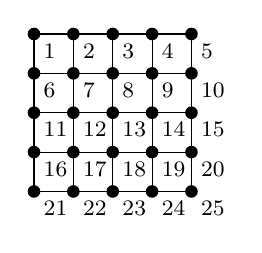
\begin{tikzpicture}
			\draw[step=.5] (0,0) grid (2,2);
			\foreach \x in {0,.5,1,1.5,2}
			\foreach \y in {0,.5,1,1.5,2}
				\fill (\x ,\y) circle (0.08);
			\node [below right] at (0,2) {\footnotesize ${1}$};
			\node [below right] at (.5,2) {\footnotesize${2}$};
			\node [below right] at (1,2) {\footnotesize${3}$};
			\node [below right] at (1.5,2) {\footnotesize${4}$};
			\node [below right] at (2,2) {\footnotesize${5}$};
			\node [below right] at (0,1.5) {\footnotesize${6}$};
			\node [below right] at (.5,1.5) {\footnotesize${7}$};
			\node [below right] at (1,1.5) {\footnotesize${8}$};			
			\node [below right] at (1.5,1.5) {\footnotesize${9}$};
			\node [below right] at (2,1.5) {\footnotesize${10}$};			
			\node [below right] at (0,1) {\footnotesize${11}$};
			\node [below right] at (.5,1) {\footnotesize${12}$};
			\node [below right] at (1,1) {\footnotesize${13}$};
			\node [below right] at (1.5,1) {\footnotesize${14}$};
			\node [below right] at (2,1) {\footnotesize${15}$};
			\node [below right] at (0,.5) {\footnotesize${16}$};
			\node [below right] at (.5,.5) {\footnotesize${17}$};
			\node [below right] at (1,.5) {\footnotesize${18}$};
			\node [below right] at (1.5,.5) {\footnotesize${19}$};
			\node [below right] at (2,.5) {\footnotesize${20}$};
			\node [below right] at (0,0) {\footnotesize${21}$};
			\node [below right] at (.5,0) {\footnotesize${22}$};
			\node [below right] at (1,0) {\footnotesize${23}$};
			\node [below right] at (1.5,0) {\footnotesize${24}$};
			\node [below right] at (2,0) {\footnotesize${25}$};
		\end{tikzpicture}
\end{figure}\

Using this system of indexing, we can find the matrix representation of the Hamiltonian. Again, the matrix is circulant; therefore, the same technique with a Discrete Fourier Transform matrix can be applied:
\newpage
\begin{theorem}
	The eigenvalues for the matrix $H$ above are
	\begin{equation}
	\lambda_t = 4 -2\cos\left(\frac{2\pi i}{M} t\right) -2\cos\left(\frac{2\pi i}{M} mt\right),
	\end{equation}
	with associated eigenvectors
	\begin{equation}
	{f}_t = (1, \omega^t, \omega^{2t}, \ldots, \omega^{(mn-1)t}) \; \; \forall t = 1, \ldots, mn.
	\end{equation}
	for $i = 1, \ldots, mn$.
\end{theorem}


\begin{proof}
	As before, columns of the DFT matrix are the eigenvectors of $H$, as shown above. The eigenvalues follow:
	\begin{align*}
	(\lambda_t f_t)_s &= (A_t f_t)_s \\
		&= 4(f_t)_s - (f_t)_{s-1} - (f_t)_{s+1} - (f_t)_{s-m} - (f_t)_{s+m} \\
		&= 4\omega^{(s-1)t} - \omega^{(s-2)t} - \omega^{st} - \omega^{(s-m-1)t} - \omega^{(s-m+1)t}
	\end{align*}
	Additionally, using the eigenvectors explicitly:
	\begin{align*}
		(\lambda_t f_t)_s &= \lambda_t (f_t)_s  \\
			&= \lambda_t \omega^{(s-1)t}
	\end{align*}
	Setting the two expressions equal, we have our eigenvalues:
	\begin{IEEEeqnarray*}{rCl}
	\lambda_t &=& 4 - \omega^{-t} - \omega^t - \omega^{-mt} - \omega^{mt}
	\\
	&=& 4 - \cos \left( -\frac{2\pi i}{M}t \right) - i \sin \left( - \frac{2\pi i}{M} t \right) - \cos \left(\frac{2\pi i}{M}t \right) - i \sin \left( \frac{2\pi i}{M} t \right)
	\\
	&& -\> \cos \left( -\frac{2\pi i}{M}mt \right) - i \sin \left( - \frac{2\pi i}{M} mt \right) - \cos \left(\frac{2\pi i}{M}mt \right) - i \sin \left( \frac{2\pi i}{M} mt \right)
	\\
	&=& 4 -2\cos\left(\frac{2\pi i}{M} t\right) -2\cos\left(\frac{2\pi i}{M} mt\right) \; \; \forall j = 1, \ldots , M,
	%4 - \cos \left( -\frac{2\pi i}{M}t \right) - \cos \left( - \frac{2\pi i}{M} j \right) - \cos \left(\frac{2\pi i}{M}j \right) - i \sin \left( \frac{2\pi i}{M} j \right) \\
% 	\lambda_t &= 4 - \omega^{-t} - \omega^t - \omega^{-mt} - \omega^{mt} \\ 	
% 	\lambda_t \omega^{(s-1)t} &= 4\omega^{(s-1)t} - \omega^{(s-2)t} - \omega^{st} - \omega^{(s-m-1)t} - \omega^{(s-m+1)t}
% 	\\ 
% 	\lambda_t = 4 - \omega^{-t} - \omega^t - \omega^{-mt} - \omega^{mt} \\
 	% 	&= 4 - \cos \left( -\frac{2\pi i}{M}t \right) - i \sin \left( - \frac{2\pi i}{M} t \right) - \cos \left(\frac{2\pi i}{M}t \right) - i \sin \left( \frac{2\pi i}{M} t \right) \\
% 			  && -\cos \left( -\frac{2\pi i}{M}mt \right) - i \sin \left( - \frac{2\pi i}{M} mt \right) - \cos \left(\frac{2\pi i}{M}mt \right) - i \sin \left( \frac{2\pi i}{M} mt \right) \\
% 			 % \cos \left( -\frac{2\pi i}{M}t \right) - i \sin \left( - \frac{2\pi i}{M} j \right) - \cos \left(\frac{2\pi i}{M}j \right) - i \sin \left( \frac{2\pi i}{M} j \right) \\
% 	  &= 2 -2\cos\left(\frac{2\pi i}{M} j\right)  \; \; \forall j = 1, \ldots , M
	\end{IEEEeqnarray*}
as desired.
\end{proof}

% Section: The Entire Infinite Two-dimensional Lattice
\section{The Entire Infinite Two-dimensional Lattice}

Our results above naturally generalize to two dimensions when the entire two-dimensional lattice (Figure~\ref{fig:2dentire}) is considered.

\begin{figure}
	\caption{The entire infinite two-dimensional lattice \label{fig:2dentire}}
	\centering
		%% To draw 2-d infinite lattice:
		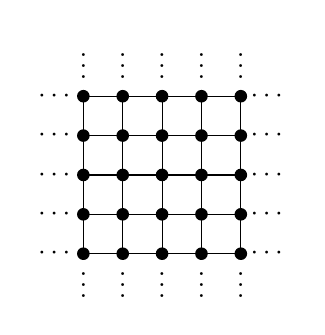
\begin{tikzpicture}
			\draw[step=.5] (0,0) grid (2,2);
			\foreach \x in {0,.5,1,1.5,2}
			\foreach \y in {0,.5,1,1.5,2}
				\fill (\x ,\y) circle (0.08);
			\foreach \y in {0,.5,1,1.5,2}
				\draw[] (2,\y) -- node[anchor=west] {{$\cdots$}} (2,\y);
			\foreach \y in {0,.5,1,1.5,2}
				\draw[] (-.7,\y) -- node[anchor=west] {{$\cdots$}} (-.7,\y);
			\foreach \x in {0,.5,1,1.5,2}
				\draw[] (\x,.1) -- node[anchor=north] {{$\vdots$}} (\x,.1);
			\foreach \x in {0,.5,1,1.5,2}
				\draw[] (\x,2.1) -- node[anchor=south] {{$\vdots$}} (\x,2.1);
		\end{tikzpicture}
\end{figure}
		
In the one-dimensional case, we found that 
	\[
	(\hl^{(1)} \psi)_x = \psi_x + \psi_{x+1} + c \psi_x
	\]
which, in terms of the basis vectors of the Hilbert space, implies that
	\begin{align}
	\label{definec}
	(\hl^{(1)} e_z)_x &= \delta_{x-1} + \delta_{x-1} + c\delta_x \notag \\
		&= e_{z+1} + e_{z-1} + ce_z.
	\end{align}
	
The two-dimensional case is analogous; for any lattice site $(x,y)$, and denoting $e_{(x,y)} = e_x \otimes e_y$, the Hamiltonian is given by
	\begin{align*}
	H^{(2)} e_{(x,y)} &= H^{(2)} (e_x \otimes e_y) \\
		&= e_{x-1} \otimes e_y + e_{x+1} \otimes e_y + e_x \otimes e_{y-1} + e_x \otimes e_{y+1} + ce_x \otimes e_y \\
		&= H^{(1)}e_x \otimes e_y - ce_x \otimes e_y + e_x \otimes H^{(1)} e_y - ce_x \otimes e_y + ce_x \otimes e_y
	\end{align*}

We can therefore factor this expression using the tensor product:
	\begin{align}
	(H^{(2)} - c \mathds{1} \otimes \mathds{1}) (e_x \otimes e_y) &= [(H^{(1)} - c\mathds{1}) \otimes \mathds{1} + \mathds{1} \otimes ({H}^{(1)} - c\mathds{1})] (e_x \otimes e_y) \nonumber \\
	(H^{(2)} - c \mathds{1} \otimes \mathds{1}) &= [(H^{(1)} - c\mathds{1}) \otimes \mathds{1} + \mathds{1} \otimes ({H}^{(1)} - c\mathds{1})]
	\end{align}

The eigenvalues of $H^{(2)}$ are easily found as a result:

\begin{theorem}

The eigenvectors for the matrix $H^{(2)}$, corresponding to the discrete second-order Laplacian on the entire two-dimensional lattice, are
\begin{equation}
	w_{kl} = v_k \otimes v_l
\end{equation}
with corresponding eigenvalues
\begin{equation}
	\eta_{kl} = \lambda_k + \lambda_l - c,
\end{equation}
where $\lambda_k$ is the eigenvalue corresponding to the eigenvector $v_k$ of the one-dimensional matrix $H^{(1)}$ and $c$ is defined in Equation~(\ref{definec}).
\end{theorem}
\begin{proof}
This follows directly from our computations above:
	\begin{align*}
	H^{(2)} w_{kl} &= (c\mathds{1} \otimes \mathds{1}) w_{kl} + (H^{(1)} - c\mathds{1}) \otimes \mathds{1} w_{kl} + \mathds{1} \otimes (H^{(1)} - c\mathds{1}) w_{kl} \\
		&= cw_{kl} + (H^{(1)} - c\mathds{1}) v_k \otimes v_l + v_k \otimes (H^{(1)} - c\mathds{1})v_l \\
		&= cw_{kl} + (\lambda_k - c) v_k \otimes v_l + v_k \otimes (\lambda_l - c)v_l \\
		&= cw_{kl} + (\lambda_k - c) w_{kl} + (\lambda_l - c)w_{kl} \\
		&= (\lambda_k + \lambda_l - c) w_{kl},
	\end{align*}
as desired.
\end{proof}

% Section: Existence of the Zero Ground State
\section{Existence of the Zero Ground State}

Next, we wish to begin considering half-infinite lattices with differing types of boundaries. Another author considers a boundary of slope 0, with respect to the $x$-axis, as shown in Figure~\ref{slope0} \cite{young}.

\begin{figure}
	\caption{Half-infinite lattice with boundary slope of 0 		\label{slope0}}
	\centering
		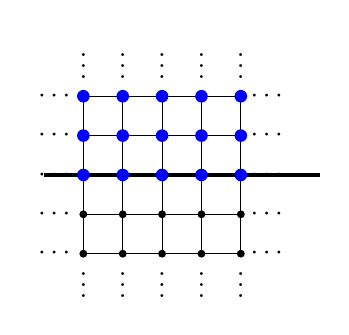
\begin{tikzpicture}
			\draw[step=.5] (0,0) grid (2,2);
			\foreach \x in {0,.5,1,1.5,2}
			\foreach \y in {0,.5,1,1.5,2}
				\fill (\x ,\y) circle (0.05);
			\foreach \y in {0,.5,1,1.5,2}
				\draw[] (2,\y) -- node[anchor=west] {{$\cdots$}} (2,\y);
			\foreach \y in {0,.5,1,1.5,2}
				\draw[] (-.7,\y) -- node[anchor=west] {{$\cdots$}} (-.7,\y);
			\foreach \x in {0,.5,1,1.5,2}
				\draw[] (\x,.1) -- node[anchor=north] {{$\vdots$}} (\x,.1);
			\foreach \x in {0,.5,1,1.5,2}
				\draw[] (\x,2.1) -- node[anchor=south] {{$\vdots$}} (\x,2.1);
			\draw[very thick](-.5,1)--(3,1);
			\foreach \x in {0,.5,1,1.5,2}
			\foreach \y in {1,1.5,2}
				\fill[color=blue](\x,\y) circle(0.08);
		\end{tikzpicture}
\end{figure}

We shall extend this investigation to consider two similar, but distinct, two-dimensional half-infinite lattices in this paper, with boundary slopes of $1$ and $2$. These correspond to boundary angles of $\arctan (1) = \pi/4 = 45\degree$ and $\arctan (2) \approx 1.11 \approx 63.43 \degree$ (relative to the $x$-axis), respectively.

Before we do so, however, it is useful to state and prove a general theorem guaranteeing the existence of a zero eigenvalue for the cases we consider.

First, we generalize the second-order discrete Laplacian, the Hamiltonian operator we have been using up until this point, by allowing two parameters (those quantifying nearest-neighbor interactions) to vary:

\begin{definition}
Define the generalized second-order discrete Laplacian Hamiltonian $\tilde{H}_\Lambda$ by
\[
\tilde{H}_\Lambda = \sum_{x \twoheadrightarrow y} h_{xy},
\]
where the summation is over all directed edges $\xyedge$ for $x,y \in \Lambda$, and
\[
\label{newham}
h_{xy} = \left\{
	\begin{array}{ll}
		\Ket{ \lambda_h e_x - e_y } \Bra { \lambda_h e_x - e_y } & \textnormal{ if } \xyedge \textnormal{ is horizontal} \\
		\Ket{ \lambda_v e_x - e_y } \Bra { \lambda_v e_x - e_y } & \textnormal{ if } \xyedge \textnormal{ is vertical}
	\end{array}
	\right.
\]
for $\lambda_h, \lambda_v \geq 0$.
\end{definition}

This definition of the Hamiltonian $\tilde{H}$ subsumes the Hamiltonian $H$ previously defined in Definition 1.1 as the special case in which $\lambda_h = \lambda_v = 1$. Accordingly, from this point forward, the operator $H$ shall refer to that defined in Definition~\ref{newham}. In addition, all Hamiltonians of this class are positive semidefinite, as defined as follows:

\begin{definition}
A matrix is positive semidefinite (denoted $A \geq 0$) if $A^* = A$ and $\langle \psi, A \psi \rangle \geq 0$ for all vectors $\psi$.
\end{definition}

A very useful property of positive semidefinite matrices is that all of its eigenvalues are non-negative. In addition, the following Lemma provides another useful property:
\begin{lemma}
For positive semidefinite matrices $A_i \geq 0, i = 1, ..., N$,
\[
\left(\sum_{i = 1}^N A_i\right) \psi = 0 
\]
if and only if $A_i \psi = 0$ for all $ i = 1, ..., N$.
\end{lemma}

\begin{proof}
% 	Suppose $A_1, A_2$ are positive semidefinite matrices and $(A_1 + A_2)\psi = 0$. Then, $\psi^T{}(A_1 + A_2) \psi = 0$. Because $A_1, A_2$ are positive semidefinite, we know that $\psi^T{} A_1 \psi, \psi^T{} A_2 \psi \geq 0$, so it must follow that $\psi^T{} A_1 \psi = \psi^T{} A_2 \psi = 0$.
% 	It remains to show that for a positive semidefinite matrix $A$, $\psi^T{} A \psi$ = 0 implies that $ A \psi$ = 0. 
% 	Now, suppose that for a positive semidefinite matrix $A$, $\psi^T{} A \psi = 0$ and $ A \psi \neq 0$. Because $A$ is positive semidefinite, there exists $B$ such that $A = B^T{} B$. Then, $\psi^T{} B^T{} B \psi = (B \psi)^T{} B \psi = 0$, which implies that $B \psi = 0$ (since a self-orthogonal vector is a zero vector, by definition). But then $A\psi = B^T{} B\psi = 0$.
	%Then, $\psi \neq 0$ and $\psi \perp A \psi$, implying that $(A \psi)^T{} \psi$
	%, i.e., $\psi^T{} A_1 \psi = \psi^T{} A_2 \psi = 0$
	Suppose $A_1, A_2$ are positive semidefinite matrices and $(A_1 + A_2)\psi = 0$. Then, $\psi^T{}(A_1 + A_2) \psi = 0$. Because $A_1, A_2$ are positive semidefinite, we know that $\psi^T{} A_1 \psi, \psi^T{} A_2 \psi \geq 0$, so it must follow that $\psi^T{} A_1 \psi = \psi^T{} A_2 \psi = 0$. Because $A_1$ is positive semidefinite, there exists $B$ such that $A_1 = B^T{} B$. Then, $\psi^T{} B^T{} B \psi = (B \psi)^T{} B \psi = 0$, which implies that $B \psi = 0$ (since a self-orthogonal vector is a zero vector, by definition). But then $A_1\psi = B^T{} B\psi = 0$. The case for $A_2 \psi$ is analogous. The generalization to an arbitrary number of matrices $A_i$ follows by induction, and the reverse direction of the lemma is trivial.
\end{proof}

These properties help us prove the main theorem of this section:

\begin{theorem}
	For any finite, connected lattice such that $\lambda_h, \lambda_v > 0$, there will exist a unique ground state (i.e., there will exist exactly one $\psi$ such that $\hl \psi$ = 0), up to normalization.
\end{theorem}

\begin{proof}
By the lemma above, $H_\Lambda \psi =\left( \sum_{\xyedge} h_{xy} \right) \psi = 0$ if and only if $h_{xy} = 0$ for all directed $\xyedge$ of the lattice $\Lambda$. It thus suffices to show that there exists a unique solution $\psi$, up to normalization, of the equations $h_{xy} = 0$, i.e.,



\begin{IEEEeqnarray}{rCl}
	h_{xy} \Ket{\psi} &=& \lambda^2 \Ket{e_x} \Braket{e_x |\psi_x e_x} + \Ket{e_y} \Braket{e_y | \psi_x e_x} 
	\\ && -\> \lambda \Ket{e_x} \Braket{e_y | \psi_y e_y} - \lambda \Ket{e_y} \Braket{e_x | \psi_x e_x} \nonumber
	\\
	&=& \psi_x \lambda^2 \Ket{e_x} + \psi_y \Ket{e_y} - \lambda \psi_y \Ket{e_x} - \lambda \psi_x \Ket{e_y} \nonumber
	\\
	&=& 0, \nonumber
\end{IEEEeqnarray}
where $\lambda$ represents either $\lambda_v$ or $\lambda_h$, whichever applies, depending upon whether $x$ and $y$ are joined horizontally or vertically.
Express $\psi$ in the canonical basis:
\[
\psi = \sum_{x = 1}^{|\Lambda|} \psi_x \Ket {e_x}
\]
Then, for any $\xyedge$, $h_{xy} = 0$ if and only if $\lambda \psi_x - \psi_y = 0$, or
\begin{equation}
\label{lambdarelation}
\lambda \psi_x = \psi_y.
\end{equation}
(Again,  here $\lambda$ represents either $\lambda_v$ or $\lambda_h$, as appropriate.)

Now, we assumed that $\Lambda$ is a connected lattice. Hence, if the set of equations given by Equation~\ref{lambdarelation} is consistent for all edges, then fixing one value $\psi_1$ will uniquely determine all other components of $\psi$.

To see that consistency indeed holds, we observe that Equation~\ref{lambdarelation} simply states that, when moving one lattice site up (resp. to the right), the value of the corresponding component of $\psi$ will be multiplied by a factor of $1/\lambda_v$ (resp. $1/\lambda_h$). Since $\lambda_v, \lambda_h$ do not depend upon the lattice sites $x$ or $y$ involved, the successive multiplications and divisions imply that the resulting relation between the components corresponding to any two lattice sites $z_1, z_2 \in \Lambda$ will be independent of the path taken between them.

\end{proof}

% Section: A Conjecture on the Relationship between Bound States and Spectral Gaps
\section[A Conjecture on the Relationship between Bound States \\ and Spectral Gaps]{\sloppy A Conjecture on the Relationship between Bound States and Spectral Gaps}
%\addcontentsline{toc}{section}{\protect\numberline{7}{A Conjecture on the Relationship between Bound States \\ and Spectral Gaps}}

Let us briefly revisit the model we considered in Section 3.2, in which we perturbed a one-dimensional free-end chain with a varying constant $c = b - a$. According to Proposition 3.3, this results in a bound state exactly when the absolute value of the perturbation is greater than 1. We can also examine the spectral properties resulting from this perturbation. Figure~\ref{boundstateperturb} shows the eigenvalues of the perturbed Hamiltonian as functions of the value of the perturbation $c$. Observe that at $c$ = 1, the ground state eigenvector begins to separate from the rest of the continuous spectrum, resulting in a spectral gap.
\begin{figure}
\caption{Bound state of the model in Section 3.2 when perturbed	\label{boundstateperturb}}
\includegraphics[scale=0.6]{../Matlab/URCdemo/plot_bound_states_centerperturb_20x20_bysizeofc_20140424}
\end{figure}

We now consider whether these two phenomena---the beginning of a spectral gap and the beginning of the appearance of a bound state---are related to each other. Formally, we wish to test the following:
\begin{conjecture}
	The conditions under which the spectral gap appears are also the conditions under which bound states exist.
\end{conjecture}
To test this conjecture, we consider the two aforementioned different half-infinite lattices, each with a different boundary:
\begin{enumerate}
	\item \textbf{Boundary slope 1:} This lattice, depicted in Figure \ref{slope1},  has a boundary angle of $\arcsin(1) = 45\degree$.
	\item \textbf{Boundary slope 2:} This lattice, depicted in Figure \ref{slope2},  has a boundary angle of $\arcsin(2) \approx 63\degree$.
\end{enumerate}

% Figure: Half-infinite lattices (slopes 1 and 2)
\begin{figure}
	\caption{Half-infinite lattices with boundary slopes of $1$ and $2$}
	\centering
	\begin{subfigure}{.4\linewidth}
		\caption{Boundary slope $1$		\label{slope1}}
		
	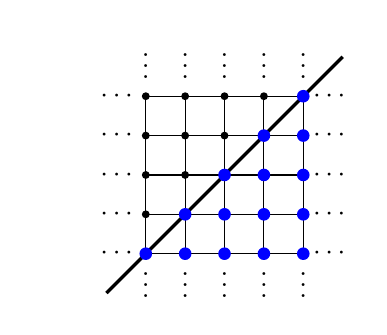
\begin{tikzpicture}
	\centering
	\path (-15mm,0);
			\draw[step=.5] (0,0) grid (2,2);
			\foreach \x in {0,.5,1,1.5,2}
			\foreach \y in {0,.5,1,1.5,2}
				\fill (\x ,\y) circle (0.05);
			\foreach \y in {0,.5,1,1.5,2}
				\draw[] (2,\y) -- node[anchor=west] {{$\cdots$}} (2,\y);
			\foreach \y in {0,.5,1,1.5,2}
				\draw[] (-.7,\y) -- node[anchor=west] {{$\cdots$}} (-.7,\y);
			\foreach \x in {0,.5,1,1.5,2}
				\draw[] (\x,.1) -- node[anchor=north] {{$\vdots$}} (\x,.1);
			\foreach \x in {0,.5,1,1.5,2}
				\draw[] (\x,2.1) -- node[anchor=south] {{$\vdots$}} (\x,2.1);
			\draw[very thick](-.5, -.5)--(2.5,2.5);
			\fill [color=blue] (0,0) circle (0.08);
			\fill [color=blue] (.5,0) circle (0.08);
			\fill [color=blue] (1,0) circle (0.08);
			\fill [color=blue] (1.5,0) circle (0.08);
			\fill [color=blue] (2,0) circle (0.08);
			\fill [color=blue] (.5,.5) circle (0.08);
			\fill [color=blue] (1,.5) circle (0.08);
			\fill [color=blue] (1.5,.5) circle (0.08);
			\fill [color=blue] (2,.5) circle (0.08);
			\fill [color=blue] (1,1) circle (0.08);
			\fill [color=blue] (1.5,1) circle (0.08);
			\fill [color=blue] (2,1) circle (0.08);
			\fill [color=blue] (1.5,1.5) circle (0.08);
			\fill [color=blue] (2,1.5) circle (0.08);
			\fill [color=blue] (2,2) circle (0.08);
	\end{tikzpicture}
	\end{subfigure}
	\begin{subfigure}{.4\linewidth}
		\caption{Boundary slope $2$	\label{slope2}}
		
	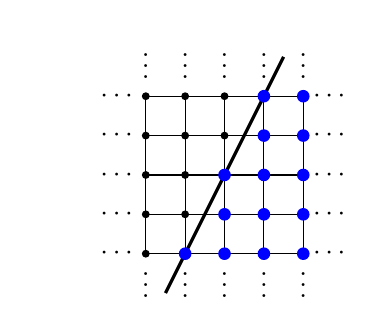
\begin{tikzpicture}
	\centering
	\path (-15mm,0);
			\draw[step=.5] (0,0) grid (2,2);
			\foreach \x in {0,.5,1,1.5,2}
			\foreach \y in {0,.5,1,1.5,2}
				\fill (\x ,\y) circle (0.05);
			\foreach \y in {0,.5,1,1.5,2}
				\draw[] (2,\y) -- node[anchor=west] {{$\cdots$}} (2,\y);
			\foreach \y in {0,.5,1,1.5,2}
				\draw[] (-.7,\y) -- node[anchor=west] {{$\cdots$}} (-.7,\y);
			\foreach \x in {0,.5,1,1.5,2}
				\draw[] (\x,.1) -- node[anchor=north] {{$\vdots$}} (\x,.1);
			\foreach \x in {0,.5,1,1.5,2}
				\draw[] (\x,2.1) -- node[anchor=south] {{$\vdots$}} (\x,2.1);
%			\draw[very thick](.5,0)--(1.5,2);
			\draw[very thick](.25,-.5)--(1.75,2.5);
			\fill [color=blue] (.5,0) circle (0.08);
			\fill [color=blue] (1,0) circle (0.08);
			\fill [color=blue] (1.5,0) circle (0.08);
			\fill [color=blue] (2,0) circle (0.08);
			\fill [color=blue] (1,.5) circle (0.08);
			\fill [color=blue] (1.5,.5) circle (0.08);
			\fill [color=blue] (2,.5) circle (0.08);
			\fill [color=blue] (1,1) circle (0.08);
			\fill [color=blue] (1.5,1) circle (0.08);
			\fill [color=blue] (2,1) circle (0.08);
			\fill [color=blue] (1.5,1.5) circle (0.08);
			\fill [color=blue] (1.5,2) circle (0.08);
			\fill [color=blue] (2,1.5) circle (0.08);
			\fill [color=blue] (2,2) circle (0.08);
	\end{tikzpicture}
	\end{subfigure}
\end{figure}

We proceed with analyzing the first lattice in close detail.

% Section: The Half-infinite Two-dimensional Lattice with Boundary Slope 1
\section[The Half-infinite Two-dimensional Lattice with \\ Boundary Slope~1]{\sloppy The Half-infinite Two-dimensional Lattice with Boundary Slope~1}
%\addcontentsline{toc}{section}{\protect\numberline{8}{The Half-infinite Two-dimensional Lattice with Boundary \\ Slope 1}}

To model the behavior of an infinite two-dimensional half-infinite lattice with a boundary slope of 1, we construct triangle lattices with such a boundary, with the points labeled as in Figure \ref{fig:label45}.

\begin{figure}
	\caption{Half-infinite lattice with boundary slope 1 with sites labeled	\label{fig:label45}}
	\centering
	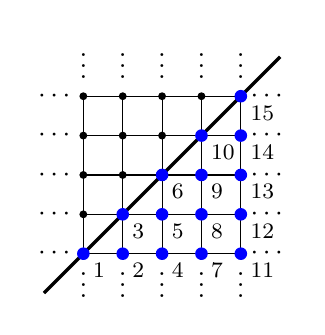
\begin{tikzpicture}
			\draw[step=.5] (0,0) grid (2,2);
			\foreach \x in {0,.5,1,1.5,2}
			\foreach \y in {0,.5,1,1.5,2}
				\fill (\x ,\y) circle (0.05);
			\foreach \y in {0,.5,1,1.5,2}
				\draw[] (2,\y) -- node[anchor=west] {{$\cdots$}} (2,\y);
			\foreach \y in {0,.5,1,1.5,2}
				\draw[] (-.7,\y) -- node[anchor=west] {{$\cdots$}} (-.7,\y);
			\foreach \x in {0,.5,1,1.5,2}
				\draw[] (\x,.1) -- node[anchor=north] {{$\vdots$}} (\x,.1);
			\foreach \x in {0,.5,1,1.5,2}
				\draw[] (\x,2.1) -- node[anchor=south] {{$\vdots$}} (\x,2.1);
			\draw[very thick](-.5, -.5)--(2.5,2.5);
			\fill [color=blue] (0,0) circle (0.08);
			\fill [color=blue] (.5,0) circle (0.08);
			\fill [color=blue] (1,0) circle (0.08);
			\fill [color=blue] (1.5,0) circle (0.08);
			\fill [color=blue] (2,0) circle (0.08);
			\fill [color=blue] (.5,.5) circle (0.08);
			\fill [color=blue] (1,.5) circle (0.08);
			\fill [color=blue] (1.5,.5) circle (0.08);
			\fill [color=blue] (2,.5) circle (0.08);
			\fill [color=blue] (1,1) circle (0.08);
			\fill [color=blue] (1.5,1) circle (0.08);
			\fill [color=blue] (2,1) circle (0.08);
			\fill [color=blue] (1.5,1.5) circle (0.08);
			\fill [color=blue] (2,1.5) circle (0.08);
			\fill [color=blue] (2,2) circle (0.08);
			\node [below right] at (0,0) {\footnotesize ${1}$};
			\node [below right] at (.5,0) {\footnotesize${2}$};
			\node [below right] at (.5,.5) {\footnotesize${3}$};
			\node [below right] at (1,0) {\footnotesize${4}$};
			\node [below right] at (1,.5) {\footnotesize${5}$};
			\node [below right] at (1,1) {\footnotesize${6}$};
			\node [below right] at (1.5,0) {\footnotesize${7}$};
			\node [below right] at (1.5,.5) {\footnotesize${8}$};			
			\node [below right] at (1.5,1) {\footnotesize${9}$};
			\node [below right] at (1.5,1.5) {\footnotesize${10}$};			
			\node [below right] at (2,0) {\footnotesize${11}$};
			\node [below right] at (2,.5) {\footnotesize${12}$};
			\node [below right] at (2,1) {\footnotesize${13}$};
			\node [below right] at (2,1.5) {\footnotesize${14}$};
			\node [below right] at (2,2) {\footnotesize${15}$};
	\end{tikzpicture}
\end{figure}

The total number of points for such a lattice $\Lambda$ of $n$ columns and rows is given by the $n$-th triangular number, i.e.,
\begin{equation}
	|\Lambda| = \binom{n}{2}.
\end{equation}
For example, for the lattice in Figure \ref{fig:label45}, the total number of lattice points is
\[
	|\Lambda| = \binom{5}{2} = 20.
\]
For sake of simplicity, the remainder of this paper shall refer to this $n$ (the number of columns in the lattice) as the lattice size instead of the actual number of points in the lattice.

In this case, instead of considering perturbations, we shall be interested in when and how the two parameters $\lambda_v$ and $\lambda_h$ of the generalized Laplacian operator affect the existence of a bound state or a spectral gap for that operator.

To test our conjecture, there are two properties of any Hamiltonian pertaining to this lattice that we must know: the spectral gap, and the existence or absence of a bound state.

The spectral gap of a matrix $H$ is defined as the difference between the two smallest eigenvalues of $H$. (Recall that, for our purposes, $H$ is always Hermitian, and hence all its eigenvalues are real; as a result, ``small'' makes sense in this context.) According to Theorem 6.1, the smallest eigenvalue for the cases we consider here is always $0$; hence, the spectral gap is simply the second smallest eigenvalue.

Determining whether the ground state is also a bound state, however, is not quite so straightforward. Since we are considering finite lattices as an approximation of their half-infinite counterparts, we will not have any wavevectors that are divergent in the 2-norm (i.e., there will exist no $\psi$ such that $\psi \in \ell^\infty(\Lambda)$ but $\psi \notin \ell^2(\Lambda)$). We will therefore consider the following quantity, which (for lack of a better name) shall be called the ``norm ratio'', as a function of the ground state eigenvector $\widetilde{\psi}$:
\begin{equation}
\label{normration}
R(\widetilde{\psi}) = \frac{||\widetilde{\psi}||_\infty}{||\widetilde{\psi}||_2}.
\end{equation}
If this quantity approaches $0$ as the size of the lattice increases, then the 2-norm grows faster than the $\infty$-norm. This would appear to indicate that as the lattice becomes larger (and hence, $\widetilde{\psi}$ becomes longer), there will be terms toward the end of the vector sufficiently large to overpower the previous terms, suggesting divergence of $\widetilde{\psi}$ in the 2-norm. If true, this would correspond to a scattering state.

On the other hand, if this quantity approaches some constant $\xi \neq 0$ as the size of the lattice increases, then it would appear that the larger terms in $\widetilde{\psi}$ appear toward the beginning of the vector, which would suggest convergence of the 2-norm and, thus, membership in the $\ell^2$ space, and would correspond to a bound state.

Although it is not difficult to construct a matrix representation of the Hamiltonian for this lattice (or, for that matter, any other lattices considered in this paper), it is not immediately obvious how such matrices could be diagonalized analytically (e.g., by the methods considered in previous sections). However, both of the key quantities just described---the spectral gap and the norm ratio---can be readily calculated numerically by MATLAB. Accordingly, our analysis from this point on will rely heavily upon such computations. (Code for all of the MATLAB routines necessary to replicate these results is given in the Appendix.)

As our first step, we need to determine how large of a lattice we need to use in our computations. To do this, we plot the norm ratio $R(\widetilde{\psi})$ against $n$ (the number of columns in the lattice) for various values of $\lambda_v$ and $\lambda_h$. This is shown in Figure \ref{fig:45howbig}. We look for a value of $n$ at which point we can reasonably expect to be able to differentiate between bound state vectors and continuous spectrum vectors. From this figure, $n = 30$ appears to be a reasonable choice.

Next, we examine the spectral properties and probable bound states of the Hamiltonian for various values of $\lambda_h$ and $\lambda_v$. These are also best examined with plots. Figure~\ref{fig:45normratios} gives the norm ratios, and Figure~\ref{fig:45spectralgaps} gives the spectral gaps, of Hamiltonians with varying parameter values.

\begin{figure}[p!]
	\centering
	\caption{Norm ratio by $n$ for various values of $\lambda_h$ and $\lambda_v$ (slope = 1)	\label{fig:45howbig}}
	\includegraphics[scale=0.5]{../Matlab/plot_normratio_vs_n_different_lambdas_20140609}	
\end{figure}
\begin{figure}[p!]
	\centering
	\caption{Norm ratios for various values of $\lambda_h$ and $\lambda_v$ (size = 30, slope = 1)	\label{fig:45normratios}}
	\includegraphics[scale=0.5]{../Matlab/plot_normratio_vs_lambdah_different_lambdav_20140609.png}
\end{figure}

\begin{figure}[p!]
	\centering
	\caption{Spectral gaps for various values of $\lambda_h$ and $\lambda_v$ (size = 30, slope = 1)	\label{fig:45spectralgaps}}
	\includegraphics[scale=0.6]{../Matlab/plot_spectralgap_vs_lambdah_different_lambdav_20140609.png}
\end{figure}

These figures together show that for the $\lambda_h$, $\lambda_v$ values attempted, the minimum spectral gap is indeed the location at which the norm ratio is the smallest.

With this information, it is possible to classify, for each $(\lambda_h, \lambda_v)$ pair, whether the particle will tend to be localized in a bound state, and furthermore, how it will tend to be localized. From experimental data, it appears that the particle has seven different general types of behaviors, as illustrated in Figures~\ref{fig:45d} through \ref{fig:45s}, depending upon the values of $\lambda_h, \lambda_v$:

\begin{enumerate}
	\item The particle is localized on the diagonal boundary (Figure~\ref{fig:45d}).
	\item The particle is localized on the upper right corner (Figure~\ref{fig:45f}).
	\item The particle is localized on the right boundary (Figure~\ref{fig:45r}).
	\item The particle is localized on the lower right corner (Figure~\ref{fig:45e}).
	\item The particle is localized on the lower boundary (Figure~\ref{fig:45b}).
	\item The particle is localized on the lower left corner (Figure~\ref{fig:45c}).
	\item The particle does not localize and remains in a scattered state (Figure~\ref{fig:45s}).
\end{enumerate}

For an intuitive view of how the $\lambda_h$, $\lambda_v$ parameters affect the behavior of the particle, Figure~\ref{fig:45phase} classifies the behavior of the particle at values of $\lambda_h$, $\lambda_v$ between $0.1$ and $2$ based upon visual inspection. The seven types of behaviors listed above correspond to the following symbols, respectively:
\begin{enumerate}
	\item Yellow ``x'' denotes localization on the diagonal boundary.
	\item Blue square denotes localization on the upper right corner.
	\item Pink star denotes localization on the right boundary.
	\item Red triangle denotes localization on the lower right corner.
	\item Cyan asterisk denotes localization on the lower boundary.
	\item Green circles denotes localization on the lower left corner.
	\item Black diamond denotes a delocalized (scattering) state.
\end{enumerate}

\begin{figure}[p!]
	\centering
	\caption{Density plot for $\lambda_v = 1.7, \lambda_h = 0.6$ (size = 30, slope = 1)\label{fig:45d}}
	\includegraphics[scale=0.55]{{../Matlab/DensityPlot_results_for_paper/densityplot_lv_1.70_lh_0.60_n_30}.jpg}
\end{figure}
\begin{figure}[p!]
	\centering
	\caption{Density plot for $\lambda_v = 0.6, \lambda_h = 0.6$ (size = 30, slope = 1)\label{fig:45f}}
	\includegraphics[scale=0.55]{{../Matlab/DensityPlot_results_for_paper/densityplot_lv_0.60_lh_0.60_n_30}.jpg}
\end{figure}
\begin{figure}[p!]
	\centering
	\caption{Density plot for $\lambda_v = 0.4, \lambda_h = 1.0$ (size = 30, slope = 1)\label{fig:45r}}
	\includegraphics[scale=.55]{{../Matlab/DensityPlot_results_for_paper/densityplot_lv_0.40_lh_1.00_n_30}.jpg}
\end{figure}
\begin{figure}[p!]
	\centering
	\caption{Density plot for $\lambda_v = 0.6, \lambda_h = 1.6$ (size = 30, slope = 1)	\label{fig:45e}}
	\includegraphics[scale=0.55]{{../Matlab/DensityPlot_results_for_paper/densityplot_lv_0.60_lh_1.60_n_30}.jpg}
\end{figure}
\begin{figure}[p!]
	\centering
	\caption{Density plot for $\lambda_v = 1.0, \lambda_h = 1.6$ (size = 30, slope = 1)	\label{fig:45b}}
	\includegraphics[scale=0.55]{{../Matlab/DensityPlot_results_for_paper/densityplot_lv_1.00_lh_1.60_n_30}.jpg}
\end{figure}
\begin{figure}[p!]
	\centering
	\caption{Density plot for $\lambda_v = 1.6, \lambda_h = 1.6$ (size = 30, slope = 1)	\label{fig:45c}}
	\includegraphics[scale=0.55]{{../Matlab/DensityPlot_results_for_paper/densityplot_lv_1.60_lh_1.60_n_30}.jpg}
\end{figure}
\begin{figure}[p!]
	\centering
	\caption{Density plot for $\lambda_v = 1.0, \lambda_h = 1.0$ (size = 30, slope = 1)	\label{fig:45s}}
	\includegraphics[scale=0.55]{{../Matlab/DensityPlot_results_for_paper/densityplot_lv_1.00_lh_1.00_n_30}.jpg}
\end{figure}
\begin{figure}[p!]
	\centering
	\caption{Phase diagram of particle states by $\lambda_v, \lambda_h$ (size = 30, slope = 1)	\label{fig:45phase}}
	\includegraphics[scale=0.55]{{../Matlab/phase_diagram_from_matrixx_corrected_20140609}.png}
\end{figure}

% Section: The Half-infinite Two-dimensional Lattice with Boundary Slope 1
\section[The Half-infinite Two-dimensional Lattice with \\ Boundary Slope~2]{\sloppy The Half-infinite Two-dimensional Lattice with Bound\-a\-ry Slope 2}
%\addcontentsline{toc}{section}{\protect\numberline{9}{The Half-infinite Two-dimensional Lattice with Boundary \\ Slope 2}}

Our analysis for a lattice of slope 2 is similar. The number of points in a lattice of this type with $n$ columns is
\begin{equation}
	|\Lambda| = \sum_{i=1}^n (2i-1) = 2\sum_{i=1}^n (i) - n = 2 \left( \frac{n(n+1)}{2} \right) - n = n^2.
\end{equation}
Again, from Figure~\ref{fig:63howbig}, we see that a lattice of $n = 30$ columns should be sufficient for our purposes.

\begin{figure}[p!]
	\centering
	\caption{Norm ratio by $n$ for various values of $\lambda_h$ and $\lambda_v$ (slope = 2)	\label{fig:63howbig}}
	\includegraphics[scale=0.6]{../Matlab/plot_normratio_vs_n_different_lambdas_20140610_63}	
\end{figure}

Next, like before, we examine the spectral properties and probable bound states of the Hamiltonian for various values of $\lambda_h$ and $\lambda_v$. Figure~\ref{fig:63normratios} gives the norm ratios, and Figure~\ref{fig:63spectralgaps} gives the spectral gaps, of Hamiltonians with differing parameter values. Again, we observe that the minimum values of both the norm ratios and the spectral gaps appear to coincide in each case.

\begin{figure}[p!]
	\centering
	\caption{Norm ratios for various values of $\lambda_h$ and $\lambda_v$ (size = 30, slope = 2)	\label{fig:63normratios}}
	\includegraphics[scale=0.65]{../Matlab/plot_normratio_vs_lambdah_different_lambdav_20140610_63.png}
\end{figure}

\begin{figure}[p!]
	\centering
	\caption{Spectral gaps for various values of $\lambda_h$ and $\lambda_v$ (size = 30, slope = 2)	\label{fig:63spectralgaps}}
	\includegraphics[scale=0.7]{../Matlab/plot_spectralgap_vs_lambdah_different_lambdav_20140610_63.png}
\end{figure}

% Section: Conclusions
\section{Conclusions}

In this paper, we first considered several simple cases in one and two dimensions, which we solved with several different methods (Discrete Fourier Transform, transfer matrices, and \textit{Ansatz}). These results motivated the main conjecture we investigated, which we tested by varying two parameters in the Hamiltonian and observing the resulting spectral gaps and existence of bound states. The two different half-infinite lattices we considered in the latter portion of the paper seem to support the conjecture; in each of the cases, the minimal spectral gap coincides with the probable appearance of a bound state, as evidenced by the ratio of the $\infty$-norm to the $2$-norm of the ground state eigenvector. The analysis also showed the effects of varying the nearest-neighbor interaction parameters upon the spectral properties of the Hamiltonian.

We hope to extend this research in the future by exploring methods of analytically investigating lattices such as the ones we have considered in the two preceding sections. In addition, whereas in this paper we have considered lattices with boundaries of slopes $1$ and $2$, we hope in the future to be able to construct and analyze lattice boundaries of arbitrary slopes. Finally, we wish to consider other methods of approximating half-infinite lattices such as those considered here. In this paper, we have built successively larger triangles. However, it is uncertain whether this is the most suitable way to construct such lattices, and the different types of behavior of a localized particle may be fewer than the seven presented. This may become more apparent with a different way of constructing these finite lattices.

% Section: Acknowledgments
\section*{Acknowledgments}
\addcontentsline{toc}{section}{Acknowledgments}

I wish to thank Professor Bruno Nachtergaele for his most generous and patient guidance and support throughout this project. I also would like to express my appreciation for my family---A.H., A.H., A.H., and A.H.---for their support and for bearing with a often very preoccupied Aaron throughout this project, as well as C.H., J.H, J.L., M.P., and E.Y., and my fellow classmates at SIBS-NCSU 2012 (especially C.G. and J.Y.), for their continued encouragement of my mathematical endeavors. Finally, I would like to acknowledge all of the wonderful professors, instructors, and classmates I have had the opportunity to learn from during my time here at UC Davis.

% Section: References
\addcontentsline{toc}{section}{References}

\begin{thebibliography}{1}

\bibitem{cremling}
  Christian Remling, Functional Analysis: Perturbation by Compact Operators.  \url{http://www2.math.ou.edu/~cremling/teaching/lecturenotes/fa-new/ln15.pdf}
  
\bibitem{griffiths}
  David J. Griffiths, 
  \emph{Introduction to Quantum Mechanics},
  Pearson Prentice Hall, Upper Saddle River, New Jersey,
  2nd edition,
  2005.

\bibitem{fenglinetsky}
  Limeng Feng, Vadim Linetsky, Electronic Companion to ``Pricing Options in Jump-Diffusion Models: An Extrapolation Approach'', 
  \emph{Operations Research},
  56:2, ec1-ec3 (2007).

\bibitem{young}
  Amanda Young, personal communication.
\end{thebibliography}

% Section: Appendix: MATLAB Code
\section*{Appendix: MATLAB Code}
\addcontentsline{toc}{section}{Appendix: MATLAB Code}

The analysis in Sections 8 and 9 employed MATLAB extensively to compute eigenvalues, eigenvectors, norms, spectral gaps, and other properties of the Hamiltonian operators considered. This Appendix contains the code for all of the computations performed in those sections.

Note: In the following functions, the \texttt{n} parameter specifies the number of points in the lattice, rather than the number of columns like was done in the paper.

\lstinputlisting{../Matlab/PaperCode/VertexList1.m}
\lstinputlisting{../Matlab/PaperCode/VertexList2.m}
\lstinputlisting{../Matlab/PaperCode/Ham1.m}
\lstinputlisting{../Matlab/PaperCode/Ham2.m}
\lstinputlisting{../Matlab/PaperCode/GroundState.m}
\lstinputlisting{../Matlab/PaperCode/NormRatio.m}
\lstinputlisting{../Matlab/PaperCode/ReturnSpectralGap.m}
\lstinputlisting{../Matlab/PaperCode/PlotSpectralGap.m}
\lstinputlisting{../Matlab/PaperCode/PlotNormRatioByN.m}
\lstinputlisting{../Matlab/PaperCode/PlotNormRatioByLambdah.m}
\lstinputlisting{../Matlab/PaperCode/DensityPlot1.m}
\lstinputlisting{../Matlab/PaperCode/MultipleDensityPlots.m}
\lstinputlisting{../Matlab/PaperCode/CreatePhaseDiagram.m}
\lstinputlisting{../Matlab/PaperCode/RecreatePhaseDiagram.m}

\end{document}